\documentclass[a4paper,titlepage,12pt]{article}
\usepackage[english]{babel}
\usepackage[latin1]{inputenc}
\usepackage[T1]{fontenc}
\usepackage{graphics}
\title{\textbf{Flat Hunt Developer Guide}}
\author{Ursina Caluori\\ \href{mailto: ucaluori@student.ethz.ch}{ucaluori@student.ethz.ch}}
\pagestyle{headings}
\usepackage{hyperref}
\hypersetup{colorlinks}
\begin{document}
  \maketitle
  \tableofcontents
  \pagebreak

  \paragraph{}
  \emph{TRAFFIC} \cite{sa05}, \emph{Touch} \cite{rk05} and \emph{Flat Hunt} is software that hopefully makes learning to program more fun and more interesting for you. \emph{TRAFFIC} is a library that supports the reading and display of public transportation systems. A library is a piece of software whose functionality can be used by other software. \emph{Flat Hunt} is an application that uses the \emph{TRAFFIC} library to model a city map. For the visualization the \emph{EiffelMedia} Library (formerly known as \emph{ESDL} \cite{tgb03}\cite{bb04}) is used. It is a strategy game, similar to Scotland Yard, but with a different background story (for more information about the story and gameplay of \emph{Flat Hunt}, read the Flat Hunt User Guide). \emph{Touch} is also an application that uses the \emph{TRAFFIC} library. For more information on \emph{TRAFFIC} and \emph{Touch}: see \cite{sa05} and \cite{rk05} or visit \htmladdnormallink{this website}{http://se.inf.ethz.ch/traffic}.\\

  This document describes how \emph{Flat Hunt} is built, what classes are important and highlights some of their features.
  
  \section{Getting Started}
    \emph{What you need for running \emph{Flat Hunt}\ldots}


\subsection{Requirements}
\begin{description}
  \item[EiffelStudio:] \url{http://www.eiffel.com/downloads/}
  \item[TRAFFIC:] \url{http://se.inf.ethz.ch/traffic/}
  \item[EiffelMedia:] \url{http://se.inf.ethz.ch/eiffelmedia/}
\end{description}

\subsection{Installation}
\emph{EiffelStudio}, as well as \emph{EiffelMedia}, come with an installer. Just follow the onscreen instructions like you would when installing any other program. No magic there..\\

\emph{TRAFFIC} does not need to be installed, just download the zip-file and unzip it to a directory of your choice.\\ 
Flat Hunt is located in the directory \texttt{traffic/example/flat\_hunt}. To get it to run, however, you'll have to compile it first.\\

For that you have to complete the following steps:

\begin {enumerate}
	\item{Start EiffelStudio}
	\item{Click on "File ->New Project...". Choose "Open existing Ace (control file)" from the dialog (see \autoref{newproject}) and click on "Next".
\begin{figure}[h]
\centerline{\hbox{  
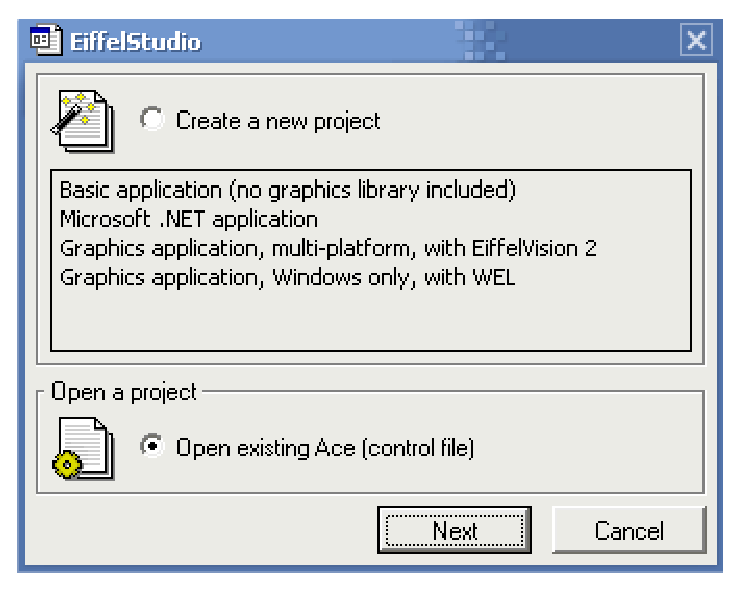
\includegraphics[width=80mm]{new_project}
  }}
\caption{New Project Dialog}
\label{newproject}
\end{figure}	  
}
	\item {This will open a file dialog that lets you choose the Ace file. Browse to the directory \texttt{traffic/example/flat\_hunt}. Depending on the operating system you are working on, choose \emph{ise\_windows.ace} or \emph{ise\_linux.ace}. Click on "Open". }
	\item{The dialog shown in \autoref{choosedir} lets you choose the project directory. In most cases you can leave both paths (Ace file and location) as EiffelStudio proposes. Make sure that the checkbox for compiling the generated project is selected. Click on "OK". This will start the compilation of the project.
\begin{figure}[h]
\centerline{\hbox{  
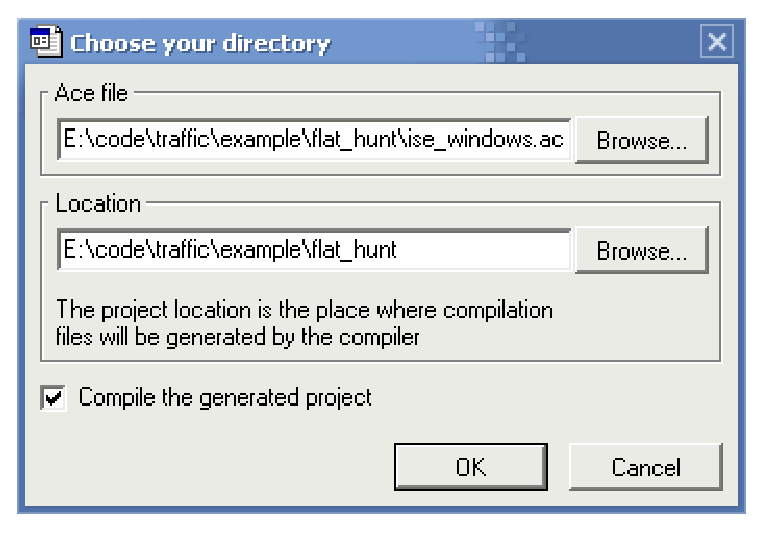
\includegraphics[width=80mm]{choose_directory}
  }}
\caption{Project Directory Dialog}
\label{choosedir}
\end{figure}
}
	\item{Once the project is compiled you can execute it by clicking on the "Launch" button in EiffelStudio or by hitting \textbf{F5}.}
\end {enumerate}

Now you are ready for playing Flat Hunt. Enjoy\ldots 



  \section{Design}
    \emph{This and the following chapter should help you understand how the Flat Hunt software is structured. This chapter will give you an overview of the whole system organization and then provide an insight to some important classes.}

\subsection{Overview}

When opening \emph{Flat Hunt} in EiffelStudio, the cluster view in the bottom left corner of EiffelStudio shows many clusters. For you only the top-level clusters \emph{Traffic} and \emph{Flat\_hunt} are important.\\

To remove complexity, \emph{Flat Hunt} is structured in three clusters (see Figure 1): \emph{Model}, \emph{View} and \emph{Controller}. In each cluster, there are several classes, and sometimes there are subclusters.\\

\subsection{Controller cluster}

Cluster Controller is the fundamental cluster in \emph{Flat Hunt}. Here are the classes that ``control'' the actions. They make sure that the displayer classes in cluster View display the proper information, which they get from the Model classes. For example, feature prepare in class \texttt{GAME} controls the display update by calling \texttt{current\_player.displayer.display\_after\_move}.

\subsection{Model cluster}
In the cluster Model, there are two important parent classes: Class \texttt{PLAYER} and class \texttt{BRAIN}. \texttt{PLAYER} is the parent of \texttt{FLAT\_HUNTER} and \texttt{ESTATE\_AGENT}, and \texttt{BRAIN} is the parent of \texttt{HUMAN}, \texttt{FLAT\_HUNTER\_BOT} and \texttt{ESTATE\_AGENT\_BOT}. These Model classes describe the internal representation of ``real world'' objects. Here is a description of some of these classes.

\subsection{View cluster}
 This clusters job is to make sure that the user sees what is going on. It includes all scenes and menus, as well as displayers for the game players and status information.

  \section{The States of the Game}
    \subsection{Overview}
Every game has at least two states: playing and game over. \emph{Flat Hunt} has six states in total; three playing states and three game over states (see Figure x). These game states are defined in class \texttt{GAME\_CONSTANTS}:

\texttt{Agent\_stuck, Agent\_stuck, Agent\_caught, Agent\_escapes, Prepare\_state, Play\_state, Move\_state: INTEGER is unique}

\begin{figure}[h]
  \centerline{\hbox{
    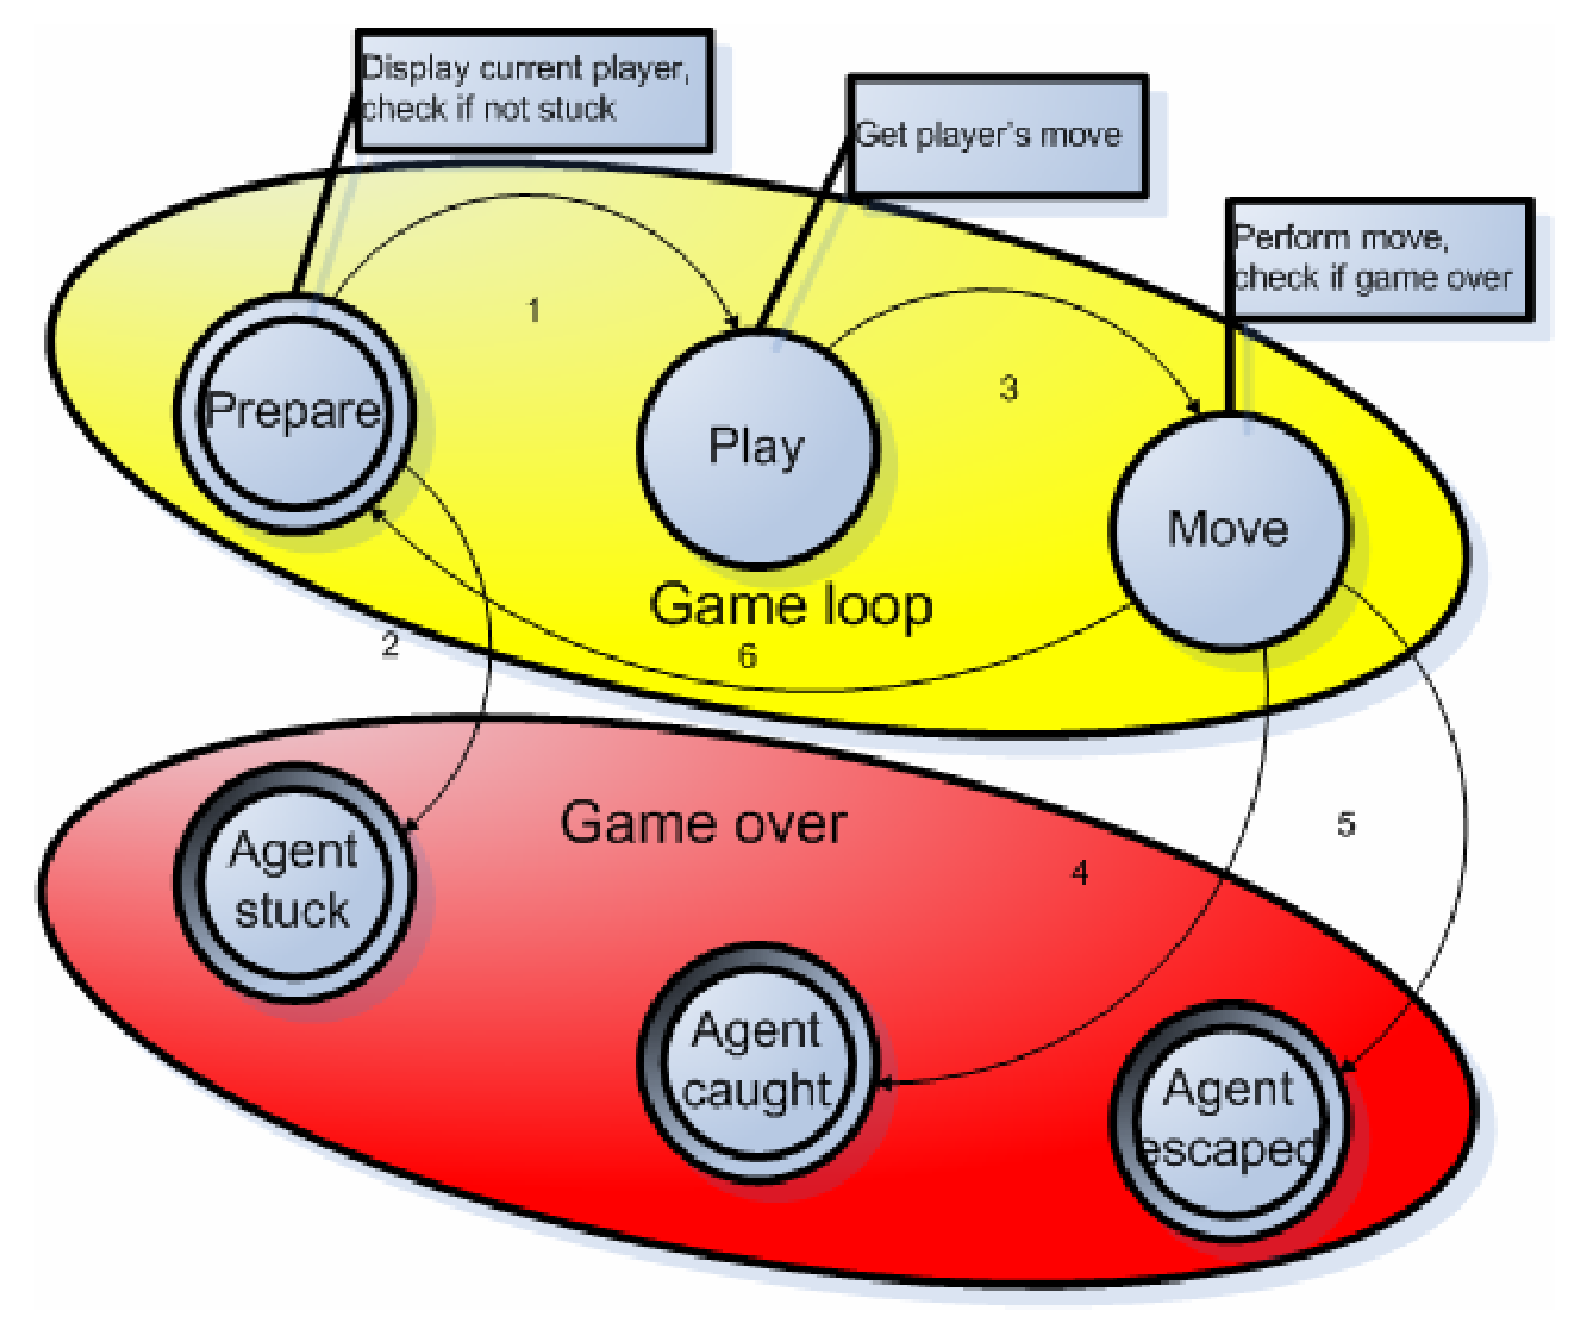
\includegraphics[width=120mm]{gameloop}
  }}
\caption{Game states and loop}
\label{gameloop}
\end{figure}

\subsection{Game Loop}
For each player in each round in \emph{Flat Hunt}, the game goes through the following states: \texttt{Prepare, Play} and \texttt{Move}. In addition, there are three game over states: \texttt{Agent\_stuck, Agent\_caught} and \texttt{Agent\_escaped}.

\begin{description}
    
  \item[Prepare] If the game is in this state, the current player gets a red circle and the possible moves are calculated and displayed. If the current player is the estate agent, and there are no possible moves, the agent is stuck and thus the game is over (state \texttt{Agent\_stuck}). If that is not the case, the game goes in state \texttt{Play}.
  
  \item[Play] In this state, if the current player is played by a human, the game waits until the human player clicks on one of the places that are highlighted. If the player is controlled by an artificial intelligence, then the best of the possible moves is calculated. The game then goes in state \texttt{Move}.
  
  \item[Move] In this state, the move selected in state \texttt{Play} is performed. After the move, the game checks if the player hits the place of the estate agent. If that is the case, the game goes into state \texttt{Agent\_caught}. If the agent did not get caught, and the round number is greater than 23, then the estate agent is the winner and the game goes into state \texttt{Agent\_escaped}. If none of the above is the case, then it's the next player's turn and the game loop starts again in state \texttt{Prepare}.

\end{description}

 
  \section{Guided ``Walk-Through''}
    \emph{What happens when you start \emph{Flat Hunt}? In this last chapter we will go step-by-step through a typical \emph{Flat Hunt} game. However, because there are lots of details involved, we concentrate on the more important steps\ldots}

\begin{enumerate}
  \item At the very beginning, the application has to be launched. By calling\\ \textit{make\_and\_launch} of the root class \texttt{FLAT\_HUNT} exactly that is achieved. This feature sets the application name, resolution and several other options and then launches the first scene to be displayed, which is of type \texttt{START} and is an heir of \texttt{START\_MENU\_SCENE}.
  \item When ``start game'' is selected in this scene, \textit{start\_callback} is called and creates a game with the proper settings and a game scene, whose job it is to visualize the game. \textit{start\_callback} also creates the \texttt{MAIN\_CONTROLLER} and calls \textit{main\_controller.start\_game}.
  \item \textit{start\_game} in class \texttt{MAIN\_CONTROLLER} calls \textit{create\_players} as well as \textit{start\_game} of class \texttt{GAME}. Those create the players using class\\ \texttt{PLAYER\_FACTORY} and set the game state to \texttt{Prepare\_state}.
  \item In class \texttt{PLAYER\_FACTORY}, for example the estate agent is created using \textit{estate\_agent.make} in feature \textit{build\_players}.
  \item This creates a \texttt{HUMAN}, \texttt{FLAT\_HUNTER\_BOT} or \texttt{ESTATE\_AGENT\_BOT} brain depending on the value of \texttt{flat\_hunters\_bot} or\\ \texttt{estate\_agent\_bot} respectively, which are boolean values to indicate if a human or the computer is going to play the corresponding player(s).
  \item Back to class \texttt{MAIN\_CONTROLLER}: Feature \textit{idle\_action} gets called whenever nothing is going on, i.e. now. \textit{idle\_action} checks whether the game is in one of the three game loop states, and calls the corresponding feature in class \texttt{MAIN\_CONTROLLER}. In the first run, this is \textit{prepare}\ldots
  \item \ldots which centers the city map on \texttt{game.current\_player} and then calls \textit{game.prepare}.
  \item \textit{prepare} of class \texttt{GAME} first calculates the estate agent's possible moves. If there are no possible moves (i.e. \texttt{current\_player.possible\_moves.\\is\_empty}) then it's either the next player's turn or the state is set to \texttt{Agent\_stuck}. Otherwise the game state is set to \texttt{Play\_state}.
  \item With that, the call to \textit{prepare} (Step 6) comes to an end and control goes back to feature \textit{idle\_action} of class \texttt{MAIN\_CONTROLLER}. According to the present game state, \textit{idle\_action} will now call \textit{play} which then calls \textit{game.play}.
  \item This calls \textit{current\_player.play (selected\_place)}, where \texttt{selected\_place} is the last place the user clicked on. \texttt{selected\_place} is then passed on to class \texttt{BRAIN}.
  \item \textit{choose\_move} in class \texttt{PLAYER} is deferred, which means that \textit{choose\_move} of class \texttt{ESTATE\_AGENT} or \texttt{FLAT\_HUNTER} gets called, depending on whether the current player is a hunter or an agent.
  \item This calls \textit{brain.choose\_move}, where brain is either a\\ \texttt{FLAT\_HUNTER\_BRAIN}, \texttt{ESTATE\_AGENT\_BRAIN} or \texttt{HUMAN}.
  \item The next move is now chosen, and thus the player moves. Control goes back to \textit{idle\_action} and we are back at step 6.
\end{enumerate}

  \section{Legal Stuff and Thanks}
    This document is based upon its prior version, which was written by Michela Pedroni and Marcel Kessler (thanks!). All graphics for the game were designed by me and Photoshop. The code of \emph{Flat Hunt} is based on its prior version \cite{mk04}, which is mainly the work of Marcel Kessler. Major parts had to be rewritten by me though.\\

Thanks to Michela Pedroni for her assistance, all my predecessors for their work, Till G. Bay (and others) for the \emph{EiffelMedia} Library (formerly \emph{ESDL} \cite{tgb03}\cite{bb04}) and Bertrand Meyer for the \emph{Eiffel} language. 


    \begin{thebibliography}{150}
    
  \bibitem{dgrk05} Roger K�ng. \emph{Touch User Guide}. ETH Zurich, 2005.\\
    \url{http://se.inf.ethz.ch/projects/roger\_kueng}
    
  \bibitem{dgsa05} Sibylle Aregger. \emph{Redesign of the TRAFFIC library}. ETH Zurich, 2005.\\
    \url{http://se.inf.ethz.ch/projects/sibylle\_aregger}
    
  \bibitem{dgrb05} Rolf Bruderer. \emph{Object-Oriented Framework for Teaching Introductory Programming}. ETH Zurich, 2005.\\
    \url{http://se.inf.ethz.ch/projects/rolf\_bruderer}
    
  \bibitem{dgmk04} Marcel Kessler. \emph{Exercise Design for Introductory Programming. "Learn-by-doing" basic OO-concepts using Inverted Curriculum}. ETH Zurich, 2004.\\
    \url{http://se.inf.ethz.ch/projects/marcel\_kessler}

  \bibitem{dgbb04} Benno Baumgartner. \emph{ESDL - Eiffel Simple Direct Media Library}. ETH Zurich, 2004.\\
    \url{http://se.inf.ethz.ch/projects/benno\_baumgartner}
    
  \bibitem{dgtgb03} Till G. Bay. \emph{Eiffel SDL Multimedia Library (ESDL)}. ETH Zurich, 2003.\\
    \url{http://se.inf.ethz.ch/projects/till\_bay}

\end{thebibliography}
    

    
\end{document}
